% --------------------------------------------------------------------------------

\begin{exercise}[272]

Betrachten Sie die folgenden Eigenschaften, die eine Menge $A$ haben kann:

\begin{enumerate}[label = \alph*.]
  \item Es gibt eine injektive Abbildung von $\omega$ nach $A$. (\Quote{$\omega \leq A$})
  \item Es gibt eine fast injektive Abbildung von $\omega$ nach $A$.
  (\Quote{fast injektiv}\ bedeutet, dass das Urbild jedes Bildpunktes endlich ist.)
  \item Es gibt eine injektive, aber nicht surjektive Abbildung von $A$ nach $A$.
  \item Es gibt eine fast injektive, aber nicht surjektive Abbildung von $A$ nach $A$.
  \item Für ein (alle) $x \notin A$ gibt es eine Bijektion von $A$ nach $A \cup \Bbraces{x}$.
  (\Quote{$A = A + 1$})
  \item Es gibt eine surjektive, aber nicht injektive Abbildung von $A$ nach $A$.
  \item Es gibt eine surjektive Abbildung von $A$ auf $\omega$. (\Quote{$\omega \leq^* A$})
  \item Es gibt eine surjektive, fast injektive Abbildung von $A$ auf $\omega$.
  \item Es gibt eine injektive Abbildung von $\omega$ nach $P(A)$. (\Quote{$\omega \leq P(A)$})
  \item Es gibt eine injektive Abbildung von $\omega$ in die endlichen Teilmengen von $A$. (\Quote{$\omega \leq P_{fin}(A)$})
  \item Es gibt eine surjektive Abbildung von den endlichen Teilmengen von $A$ auf $\omega$.
  \item $A$ ist unendlich: \Quote{$|A| = \infty$}
  \item Es gibt eine nichtleere Teilmenge von $\mathfrak{P}(A)$ ohne (bez. $\subseteq$) maximales Element.
\end{enumerate}

Geben Sie möglichst viele nichttriviale Implikationen zwischen diesen Aussagen an, die sich in ZF (also ohne Auswahlaxiom) beweisen lassen.

\end{exercise}

% --------------------------------------------------------------------------------

\begin{solution}

Es gilt die Implikationskette: a. $\implies$ b. $\implies$ c. $\implies$ d.

\begin{enumerate}[label = \arabic*.]

  \item Implikation (a. $\implies$ b.):
  
  Klar.

  \item Implikation (b. $\implies$ c.):
  
  \begin{enumerate}[label = \arabic*.]

    \item Lösung:

    Sei $f: \omega \to A$ fast injektiv.
    Wir definieren zuerst die Hilfsfunktion $k: \omega \to \omega$ durch
  
    \begin{align*}
      k(n) = \min \Bbraces{m \in \omega: \forall z < m: f(z) \neq f(m)}.
    \end{align*}
  
    Dann definiere die Funktion $g$ durch
  
    \begin{align*}
      g = \Bbraces{(x, x): x \in A \setminus f(\omega)} \cup \Bbraces{(f(n), f(n+1)): n \in \omega}.
    \end{align*}

    \item Lösung:
    
    Sei $f: \omega \to A$ fast injektiv, d.h.

    \begin{align*}
      \Forall x \in \ran f:
      |f^{-1}[\Bbraces{x}]| < \infty.
    \end{align*}

    Wir fassen $\omega$ und $A$ als Algebren mit leerem Typ auf.
    Auf diese können wir also den Homomorphiesatz anwenden und bekommen eine Abbildung $g$.

    \textbf{Achtung!}
    Möglicherweise braucht der Homomorphiesatz das Auswahlaxiom?
    Anstatt einen beliebigen Repräsentanten $u$ von $U$ zu wählen, kann man in unserem Fall den kleinsten $u := \min U$ (von endlich vielen) wählen, um $g(U) := f(u)$ zu definieren.
    Wir haben es schließlich mit Schuhen und nicht mit Socken zu tun!

    \phantom{}

    \begin{tcolorbox}[standard jigsaw, opacityback = 0]
      \centering
      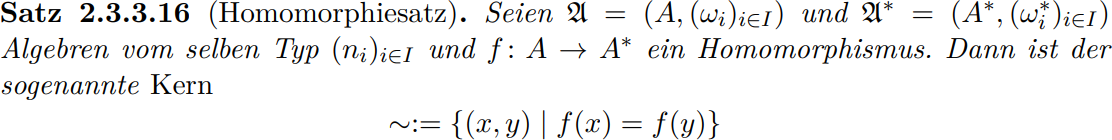
\includegraphics
      [width = 0.75 \textwidth]
      {Alg/Alg - Satz 2.3.3.16.1 (Homomorphiesatz).png} \\
      \vspace{0.25 cm}
      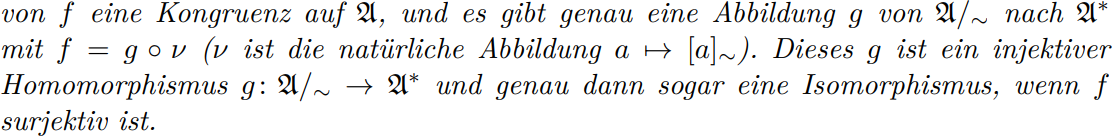
\includegraphics
      [width = 0.75 \textwidth]
      {Alg/Alg - Satz 2.3.3.16.2 (Homomorphiesatz).png} \\
      \vspace{0.25 cm}
      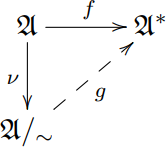
\includegraphics
      [width = 0.15 \textwidth]
      {Alg/Alg - Satz 2.3.3.16.3 (Homomorphiesatz).png}
    \end{tcolorbox}

    \phantom{}

    Seien die (unendlich vielen!) Urbilder gemäß ihrem Minimum, vermöge $h$ (strikt monoton steigend), geordnet, d.h.

    \begin{align*}
      h := (U_n)_{n \in \omega}:
      \omega \to \omega / \sim:
      \min U_1 < \min U_2 < \cdots
    \end{align*}

    $g \circ h: \omega \to A$ ist, als Verkettung injektiver Funktionen, injektiv.

  \end{enumerate}

\end{enumerate}

\end{solution}

% --------------------------------------------------------------------------------
